\chapter{Physical Loading, Diagnostic, and Spatial--Temporal Observation Laws}\label{chap:models}\label{ch:models}

The central difficulty is to separate three objects that are often conflated in stress-release modelling: the physical state that carries memory, the point process that records event occurrence, and the observation model through which events and their marks become data. The finite-mode formulation provides a transparent autonomous physical model. A diagnostic formulation specifies an independent background and separates its suppression from triggering. The distinction matters because stability, approximation and inference make different demands on the model.

\section{The physical finite-mode model}\label{sec:model_physical}

Fix a finite number of modes \(m\in\mathbb N\), with \(j\in\{1,\ldots,m\}\); every mode sum in this finite-mode model is over that set. Let \(\vartheta_j>0\) be relaxation rates and let \(w_j>0\), \(\sum_{j=1}^m w_j=1\), be fixed weights. For a constant loading \(\rho\geq0\), write
\[
x_j^*=\frac{\rho}{\vartheta_j},\qquad
\bar x=\sum_jw_jx_j^*,\qquad
\mathcal X=\left\{(Z,U):Z_j\leq x_j^*,\ U_j\geq0\right\}.
\]
The physical stress and excitation reservoir are
\begin{equation}\label{eq:physical-XH}
X=\sum_jw_jZ_j,\qquad H=\sum_jw_jU_j.
\end{equation}
Between events the coordinates relax according to
\begin{equation}\label{eq:finite-flow}
\dot Z_j=\rho-\vartheta_jZ_j,\qquad
\dot U_j=-\vartheta_jU_j.
\end{equation}
The ground event process \(N\) has compensator
\begin{equation}\label{eq:physical-compensator}
\Lambda(t)=\int_0^t\bigl\{\Psi(X(s^-))+H(s^-)\bigr\}\,\dif s .
\end{equation}
Thus the intensity is evaluated immediately before a possible event and does not include the outcome of that event.

If an event is accepted at time \(T_i\), a fresh mark \(M_i\) is drawn from a fixed law \(F\), conditionally independent of the pre-event history. Only after acceptance does the mark determine the jumps
\begin{equation}\label{eq:finite-jumps}
\Delta Z_j(T_i)=-g(M_i),\qquad
\Delta U_j(T_i)=\vartheta_j\kappa(M_i).
\end{equation}
The functions \(g,\kappa\geq0\) may depend on different aspects of the same mark and may therefore be correlated. Their first moments are denoted by
\[
m_1=\E _F g(M),\qquad n=\E _F\kappa(M).
\]
The subcritical condition \(n<1\) will control the expected branching size. Marks affect future event rates, but an accepted event cannot change the probability of its own acceptance.

The stability theorem permits a positive nondecreasing link $\Psi$ that is Lipschitz on the reached upper-bounded stress half-line. One physically signed example is
\begin{equation}\label{eq:physical-link}
\Psi(x)=e^{a+bx},\qquad b\geq0.
\end{equation}
Consequently the loading \(\rho\) acts physically through its effect on the coordinates and hence on \(X\); there is no separate multiplicative loading function in \eqref{eq:physical-compensator}. Model \eqref{eq:finite-flow}--\eqref{eq:physical-link}, with constant \(\rho\) and fixed \(\Psi\), is the autonomous finite-mode model used in the stability and approximation results.

\section{Memory kernels and exact relaxation}

For the finite-mode flow,
\begin{equation}\label{eq:finite-kernel}
\Phi(t)=\sum_jw_je^{-\vartheta_jt},\qquad
h(t)=-\Phi'(t)=\sum_jw_j\vartheta_je^{-\vartheta_jt}.
\end{equation}
Thus \(\Phi(0)=1\), \(\Phi\) is completely monotone, and \(h\) is a probability density:
\[
\int_0^\infty h(t)\,\dif t=1-\Phi(\infty)=1.
\]
For arbitrary finite initial coordinates, the coordinate solution gives
\begin{align}
X(t)&=\sum_jw_jZ_j(0)e^{-\vartheta_jt}+\rho\int_0^t\Phi(u)\,\dif u
-\sum_{0<T_i\leq t}g(M_i)\Phi(t-T_i),\label{eq:finite-X-mild}\\
H(t)&=\sum_jw_jU_j(0)e^{-\vartheta_jt}
+\sum_{0<T_i\leq t}\kappa(M_i)h(t-T_i).\label{eq:finite-H-mild}
\end{align}
The first initial term reduces to \(X_0\Phi(t)\) if every stress mode starts at \(Z_j(0)=X_0\); an analogous reduction for excitation requires equal initial excitation coordinates. The current event is excluded when intensity is evaluated at its left limit. General finite initial coordinates need the displayed mode sums.

Formulation \eqref{eq:finite-kernel} is a finite exponential mixture. A non-Markovian relaxation law is obtained by replacing the finite exponential sum with
\begin{equation}\label{eq:mittag-leffler}
\Phi(t)=E_\alpha\!\left(-(t/\tau)^\alpha\right),
\qquad 0<\alpha<1,\quad \tau>0,
\end{equation}
and setting \(h=-\Phi'\). Here \(E_\alpha(z)=\sum_{k=0}^{\infty}z^k/\Gamma(1+\alpha k)\) is the Mittag--Leffler function. For the exact kernel,
\[
\Phi(t)\sim \frac{\tau^\alpha}{\Gamma(1-\alpha)}t^{-\alpha},
\qquad
h(t)\sim \frac{\alpha\tau^\alpha}{\Gamma(1-\alpha)}t^{-1-\alpha}
\]
as \(t\to\infty\). Hence \(h\) is integrable while \(\Phi\) is not. The integrated triggering density is finite, while the integrated stress relaxation of a single release is infinite. The two memory objects therefore have different long-time integrability. The exact kernel is not, for noninteger \(\alpha\), a finite exponential mixture; it therefore carries genuine infinite-dimensional memory.

\begin{figure}[htb]
\centering
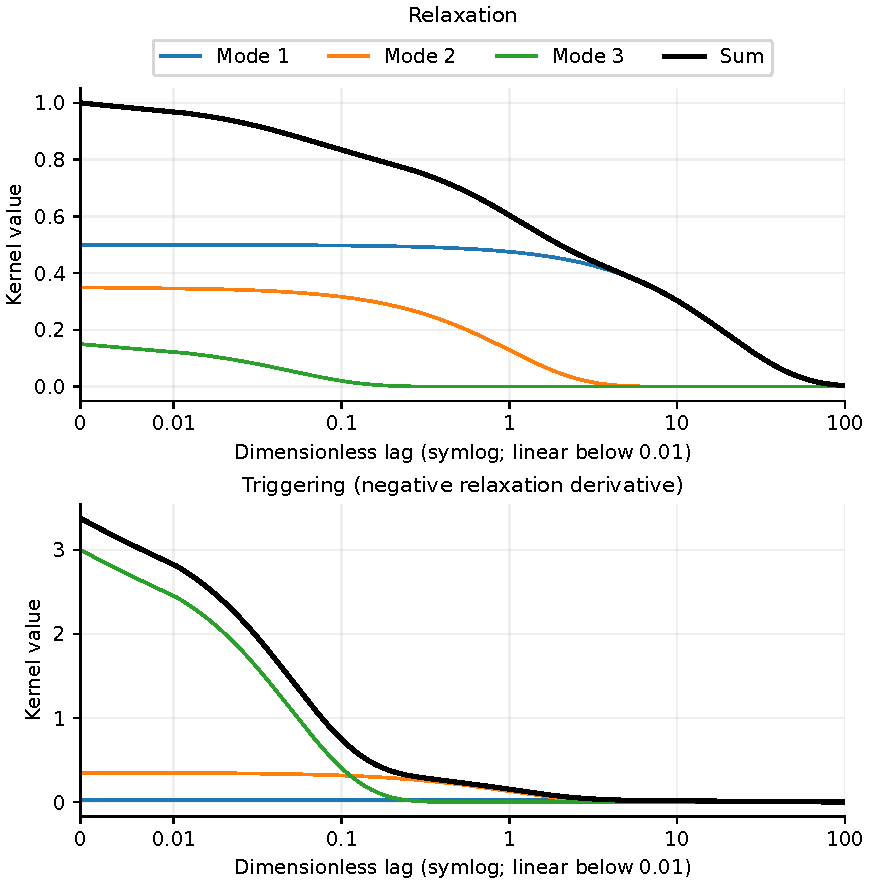
\includegraphics[width=0.95\linewidth]{finite_memory.pdf}
\caption{A dimensionless toy finite mixture with weights $(0.5,0.35,0.15)$ and rates $(0.05,1,20)$. The relaxation $\Phi$ and its negative derivative $h$ weight the same modes differently. Curves are direct evaluations of the displayed finite sums; they are not fits, simulations or an exact Mittag--Leffler kernel.}
\label{fig:finite_memory}
\end{figure}

In the physical model \(w_j\) is dimensionless, \(\vartheta_j\) and \(h\) have inverse-time units, \(\Phi\) is dimensionless, \(\rho\) is stress per unit time, and \(g(M)\) is measured in stress units. The jump \(\vartheta_j\kappa(M)\) has the units of \(U_j\). With no history, the sums in \eqref{eq:finite-X-mild}--\eqref{eq:finite-H-mild} are empty.

\section{The diagnostic model and observation}\label{sec:model_diagnostic}

For diagnostic work, retain a stress relaxation kernel \(\Phi_s\) and a normalized triggering density \(h_e\), initially allowing them to vary separately. Let \((T_i,Q_i)\) denote the accepted event times and their marks. Define the strictly prior cumulative release and excitation sums by
\begin{equation}\label{eq:diagnostic-sums}
G_s(t)=\sum_{0<T_i<t}g(Q_i)\Phi_s(t-T_i),
\qquad
H_e(t)=\sum_{0<T_i<t}\kappa(Q_i)h_e(t-T_i),
\end{equation}
and adopt the diagnostic intensity
\begin{equation}\label{eq:diagnostic-intensity}
\lambda_\eta(t)=B(t)\exp\{-\eta G_s(t)\}+nH_e(t).
\end{equation}

\begin{figure}[htb]
\centering
\includegraphics[width=0.95\linewidth]{model_architecture.pdf}
\caption{Physical loading and the independent-background diagnostic answer different questions. The left panel illustrates empty prehistory and equal initial stress coordinates $Z_j(0)=X_0$; arbitrary finite initial coordinates require the mode sum in \eqref{eq:finite-X-mild}. The physical model feeds loading through stress; the diagnostic specifies a background and suppresses its contribution by accumulated release. Triggering remains additive. The unit-productivity convention, with $n$ outside $H_e$, applies to the diagnostic.}
\label{fig:model_architecture}
\end{figure}
The baseline \(B(t)\) is deterministic at fixed parameters and specified independently of the stress-kernel family. A useful choice is \(B(t)=A\exp\{d x_{\mathrm{trend}}(t)\}\), where \(A=e^a>0\) and \(x_{\mathrm{trend}}(t)=2t/T_0-1\) for a declared fixed clock scale \(T_0>0\) (take \(T_0=T\) for the normalized single-window formulation). It is not generated by stress loading or by the marks. The strict inequalities in \eqref{eq:diagnostic-sums} are deliberate: an event is accepted before its mark is drawn, so its own release and productivity cannot enter its intensity.

This section adopts a convention change once and for all: diagnostic productivity is scaled to have unit mean,
\[
\E _F\kappa(Q)=1,
\]
while the coefficient \(n\) is retained \emph{outside} \(H_e\) in \eqref{eq:diagnostic-intensity}. In the physical model, by contrast, \(n=\E _F\kappa(M)<1\) is the mean carried by the productivity marks themselves. The diagnostic normalisation removes that mean from the marks and displays it explicitly as a coefficient. This is a bookkeeping convention, not an assertion that realised productivity is one, and it is not used to reinterpret the autonomous physical stability theorem.

The physical exponential link \eqref{eq:physical-link} embeds loading through \(X\): a constant \(\rho\) shifts the physical stress state and therefore changes \(\Psi(X)\). The time-dependent baseline \(B(t)\) in \eqref{eq:diagnostic-intensity} is an independently specified background. It does not replace \(\Psi(X)\) in the autonomous invariant-law theorem; that theorem does not cover externally varying \(B(t)\).

The shared subfamily imposes the identity \(h_e=-\Phi_s'\). This has substantive model content: the instantaneous excitation density is the negative derivative of the same kernel that governs stress relaxation. Consequently the decay of past stress and the contribution of a mark to the future compensator come from one memory structure, including its normalisation. Choices of \(\Phi_s\) and \(h_e\) that do not satisfy this identity define a separate-memory model. Normalization alone does not impose their equality.

A ground process records only the event times \(T_i\), whereas a marked process records the pairs \((T_i,Q_i)\). The ground law is a projection of the marked law. The event-time contribution to a joint marked likelihood, evaluated using observed past marks, is a different object from the marginal likelihood of times alone. Event times alone generally do not identify \(g\) and \(\kappa\) separately, nor their within-mark dependence, without an additional mark model. Conversely, the marked likelihood includes both ground acceptance probabilities and mark densities. Since marks are fresh after acceptance, past marks enter \eqref{eq:diagnostic-intensity} through the strict sums \eqref{eq:diagnostic-sums}, while a newly drawn mark first affects the future. This observational distinction is essential: marginalizing to times alone and evaluating a joint marked likelihood answer different questions.



The likelihoods studied below condition on a declared starting history. Empty prehistory is a model assumption rather than a statement that no earlier earthquakes occurred. Likewise, a fresh common mark law does not establish completeness or homogeneous measurement of the observed catalogue. Unobserved parents, omitted regions and uncertain magnitudes can change the relationship between the mathematical history and its recorded counterpart. The subsequent identification statements concern the declared complete marked process; their transfer to an earthquake catalogue requires an observation model.


\section{Master model and parameter dictionary}\label{sec:master-models}

The same letter can occur in a mathematical proof and in an archived program field. The following dictionary fixes the scientific meaning across the empirical chapters; explicitly local theoretical uses retain their stated assumptions. In particular, $X_{\rm phys}$ denotes latent physical stress when a distinction is needed, whereas $x_{\mathrm{trend}}(t)=2t/T_0-1$ is an affine clock, not a stress measurement. The earlier physical equations use $X$ for the former. A likelihood is written $\ell_{\rm score}$ when it could be confused with the LI range $\ell$; the auxiliary frozen response slope is a separate local theoretical quantity.

\begin{longtable}{@{}p{.17\textwidth}p{.77\textwidth}@{}}
\caption{Unified parameter meanings. Bounds and estimated/supplied status are procedure-specific and remain in the experimental chapters.}\label{tab:parameter-dictionary}\\
\toprule Symbol & Meaning \\\midrule\endfirsthead
\toprule Symbol & Meaning \\\midrule\endhead
$a,d$ & Log immigrant/background amplitude and affine-clock trend. Physical exponential-link slope $b$ is a different parameter. \\
$\widetilde a,\widetilde d$ & Exposure-orthogonalized background coordinates; a feasible reparameterization need not alter the represented intensity. \\
$n$ & Diagnostic excitation amplitude with unit-mean productivity; in the autonomous physical theorem it instead denotes the mean of the productivity mark. \\
$\eta$ & Nonnegative attenuation strength of the stated diagnostic history feature. \\
$\alpha,\tau$ & Mittag--Leffler fractional order and temporal scale; the implemented finite mixture is explicitly distinguished from the exact kernel. \\
$c,p$ & Omori time offset and power, with normalized density $k_O$ below. The magnitude-class cut is a separately declared threshold, not this time offset. \\
$r,\beta$ & Productivity exponent and exponential magnitude-excess rate. A training-only rate estimate and a freely fitted productivity exponent are different nuisance decisions. \\
$\omega$ & Redistribution share in the discrete spatial routing continuation. \\
$\sigma$ & Excitation spatial scale in the declared projected-domain density; a fitted/grid-selected model scale is not a measured interaction distance. \\
$\ell,\psi$ & LI attenuation range in kilometres and memory in days. Both disappear from the law at exact $\eta=0$. \\
$h,\delta$ & Magnitude-class association and parent-class fertility contrast. These do not denote the triggering density $h_e$ or a score difference $\Delta$. \\
\bottomrule
\end{longtable}

\begin{table}[htbp]\centering\small
\caption{Procedure names used in Parts III--IV. Names identify archived fitted recipes rather than new universal model families.}\label{tab:arm-dictionary}
\begin{tabularx}{\textwidth}{@{}lXX@{}}
\toprule Arm & Temporal law & Spatial/benchmark role \\\midrule
FC & Fixed-scale ML & Continuous reference-weighted offspring density \\
FL & Fixed-scale ML & Cell-lift offspring counterpart \\
MC & Free common-scale ML & Continuous offspring density \\
OC & Omori & Continuous reference-weighted offspring density \\
OL & Omori & Cell-lift offspring counterpart \\
EP & Omori ETAS adaptation & Separately fitted unweighted inverse-power radial offspring law \\
N0 & No offspring excitation & Separately refitted smooth immigrant background \\
LI & Matched OC excitation & Unrenormalized immigrant-only local attenuation \\
\bottomrule\end{tabularx}\end{table}

The labels FC through OL refer to the final smooth-background comparisons unless a factorial background is explicitly named. The earlier factorial also crosses cell and KDE-enriched backgrounds. EP is an excitation model; it is neither the no-trigger N0 recipe nor a constant-Poisson optimization floor. Comparisons of whole procedures must not be described as single-parameter inhibition ablations.

\section{Marked history and spatial observation laws}

For a magnitude excess $q$ under the working exponential law, the normalized productivity is
\[
 \kappa_r(q)=(1-r)e^{\beta rq},\qquad 0\leq r<1.
\]
Its unit mean is a property of that working law. The free-productivity experiment estimates $r$ within its declared continuous box; it is not a grid permitting $r\geq1$. The class-history extension replaces the fresh marginal mark allocation by a predictable class probability and a conditional within-class density. Its mark score includes that class probability once. Chapter~\ref{ch:temporal-extensions} gives the Perron normalization and explains why association can affect a joint fit without directly altering a fixed-history ground intensity after effective-scale matching.

On a fixed projected domain $D$, a noninhibited continuous model has
\begin{align}
 \lambda(t,z)&=e^{a+dx_{\mathrm{trend}}(t)}b_{\rm bg}(z)+nH(t,z),\label{eq:unified-spatial-law}\\
 H(t,z)&=\sum_{t_j<t}\kappa_j k_\theta(t-t_j)s_\sigma(z\mid z_j),\nonumber\\
 k_O(u)&=(p-1)c^{p-1}(u+c)^{-p},\qquad u>0,\quad c>0,\quad p>1,\nonumber\\
 s_\sigma(z\mid z_j)&=\frac{b_{\rm ref}(z)(1+\|z-z_j\|^2/\sigma^2)^{-2}}{\int_D b_{\rm ref}(v)(1+\|v-z_j\|^2/\sigma^2)^{-2}\,\dif v}.\label{eq:unified-OC-density}
\end{align}
Both spatial densities integrate to one over $D$; the temporal density integrates to one over all positive lags. Exposure uses the actual finite time window. The cell-lift counterpart allocates target-cell mass using its declared centre-based rule and spreads that mass uniformly inside the cell, retaining actual parent coordinates. EP normalizes a separately fitted radial law directly against projected area without $b_{\rm ref}$. Thus a location contrast always specifies its measure and reference.

Continuous local inhibition changes only the immigrant contribution:
\begin{align}
 \lambda_{\rm LI}(t,z)&=e^{a+dx_{\mathrm{trend}}(t)}b_{\rm bg}(z)e^{-\eta G(t,z)}+nH_{\rm OC}(t,z),\label{eq:unified-LI}\\
 G(t,z)&=\sum_{t_j<t}e^{-(t-t_j)/\psi}(1+\|z-z_j\|^2/\ell^2)^{-2}.\nonumber
\end{align}
The stress multiplier is one for every eligible recorded parent. The attenuation field is not a normalized spatial density; renormalizing the attenuated immigrant term would change the model. The observed California and synthetic-control clocks have distinct declared $T_0$, given in Chapter~\ref{ch:local-inhibition}. Exact $\eta=0$ restores OC at matching shared coordinates and makes every $\ell,\psi$ pair observationally equivalent. This boundary is the spatial counterpart of the identifiability limitation in Chapter~\ref{ch:identifiability}.

\section{Canonical proper-score semantics}\label{sec:master-scores}

Let $R(t)=\int_D\lambda(t,z)\,\dif z$ and let $\mathcal W$ be the scored window. All quantities below use the same fitted state and the same predictable observed history:
\begin{align}
 P&=\sum_{i\in\mathcal W}\log\lambda(t_i,z_i),&
 Q&=\sum_{i\in\mathcal W}\log R(t_i),\nonumber\\
 E&=\int_{\mathcal W}\int_D\lambda(t,z)\,\dif z\,\dif t,& C&=-E,\label{eq:master-PQECM}\\
 M&=\sum_{i\in\mathcal W}\log f(m_i\mid\mathcal H_{t_i},t_i,z_i).&&\nonumber
\end{align}
Thus
\begin{equation}\boxed{\begin{aligned}
 \text{Timing}&=Q+C=Q-E,\\
 \text{Conditional location}&=P-Q,\\
 \ell_{\rm score}&=P+C+M=\text{Timing}+\text{Conditional location}+M.
\end{aligned}}\label{eq:master-score-identity}\end{equation}
For temporal laws $P=Q$ and the conditional-location term is zero. For class-history laws the conditional class probability belongs to $M$, avoiding double counting. $E$ is nonnegative exposure, with expected-count dimension; it contributes negatively to a log score. A candidate-minus-reference difference obeys $\Delta C=-\Delta E$ and $\Delta\ell_{\rm score}=\Delta P+\Delta C+\Delta M$. Positive differences favour the candidate. There is no allocation of national exposure to event-only geographical groups unless an explicit spatial intensity supplies it.

\begin{table}[htbp]\centering\small
\caption{Master score-semantics crosswalk. Raw keys remain unchanged in the saved authorities; their scientific meaning is translated here.}\label{tab:score-crosswalk}
\fbox{\begin{minipage}{.94\textwidth}
\begin{tabularx}{\linewidth}{@{}XX@{}}
\toprule Saved context/key & Canonical meaning \\\midrule
Early temporal or LI pooled raw \texttt{E} & Event point-logsum contrast $\Delta P$ (temporal $\Delta Q$), not positive exposure \\
Early temporal or LI pooled raw \texttt{C} & Signed exposure contrast $\Delta C=-\Delta E$ \\
Sequence \texttt{timing\_compensator} & Difference $\Delta E$ in nonnegative exposure; it can have either sign and is subtracted \\
Benchmark \texttt{integrated\_intensity} & $E$ in arm rows, $\Delta E$ in contrast rows \\
JMA \texttt{positive\_C} / \texttt{signed\_negative\_C} & Positive exposure / its negative contribution \\
Marginal mark score & $M$, included once; it cancels only when the compared conditional mark laws agree \\
\bottomrule\end{tabularx}
\end{minipage}}
\end{table}
The pinned \path{validation/authorities/score_field_semantics_v2.json} is the documentary authority for this translation. It changes neither source fields nor scalar values. The repeated score check in Chapter~\ref{ch:design} fixes signs before any table is interpreted.
